% The two contributions on one axis: how many unknowns each inference has.
% Compile: pdflatex two_frontiers.tex && pdftocairo -svg two_frontiers.pdf two_frontiers.svg
\documentclass[tikz,border=6pt]{standalone}
\usepackage{tikz}
\usepackage{amsmath}
\usepackage{graphicx}
\usepackage[T1]{fontenc}
\usetikzlibrary{arrows.meta,calc}

\definecolor{ink}{HTML}{2E2E2E}
\definecolor{greytx}{HTML}{7A7A7A}
\definecolor{cmbc}{HTML}{C2560A}
\definecolor{lssc}{HTML}{521463}

\begin{document}
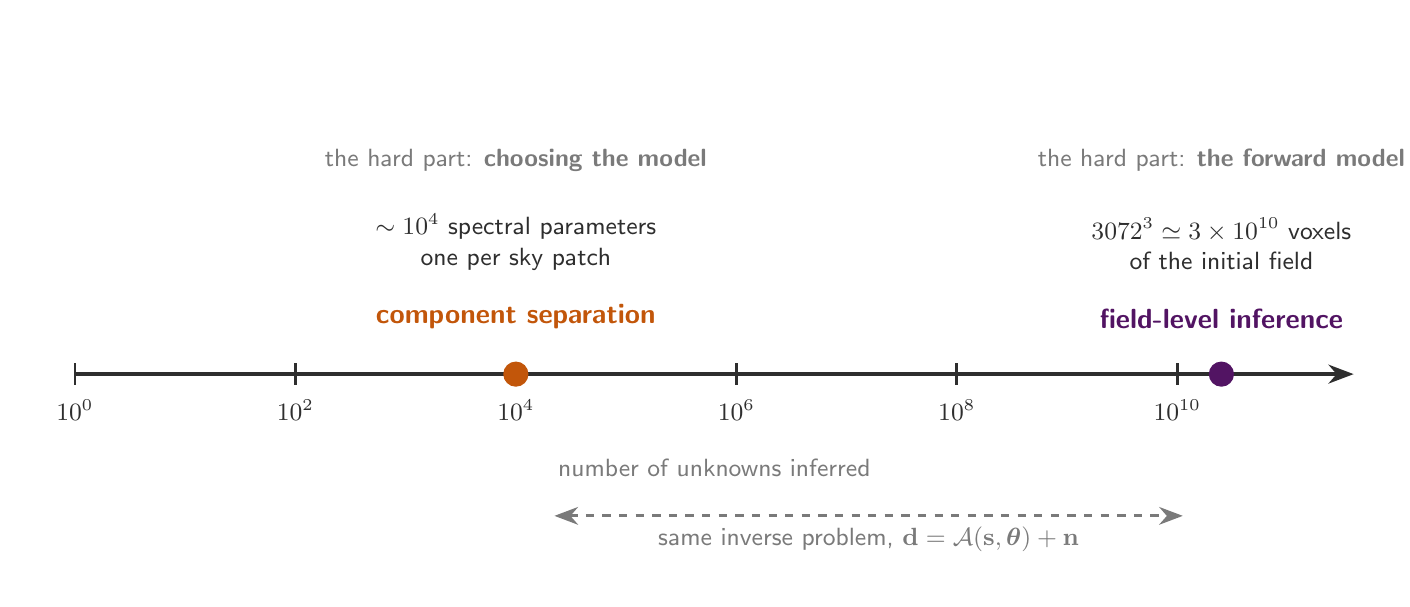
\begin{tikzpicture}[font=\sffamily]
  \useasboundingbox (-0.6,-2.6) rectangle (16.6,4.4);

  % log10 axis from 10^0 to 10^11, 1.4 cm per decade
  \def\dec{1.4}
  \draw[-{Stealth[length=3.2mm]},ink,line width=1.2pt] (0,0) -- (11.6*\dec,0);
  \foreach \p in {0,2,4,6,8,10}{
    \draw[ink,line width=1pt] (\p*\dec,0.14) -- (\p*\dec,-0.14);
    \node[ink,font=\sffamily\small,anchor=north] at (\p*\dec,-0.2) {$10^{\p}$};}
  \node[greytx,font=\sffamily\small,anchor=north] at (5.8*\dec,-0.95)
       {number of unknowns inferred};

  % Contribution 1: spectral parameters, ~10^4
  \fill[cmbc] (4*\dec,0) circle (0.16);
  \node[cmbc,font=\sffamily\bfseries,anchor=south,align=center] at (4*\dec,0.45)
       {component separation};
  \node[ink,font=\sffamily\small,anchor=south,align=center] at (4*\dec,1.2)
       {$\sim 10^{4}$ spectral parameters\\one per sky patch};
  \node[greytx,font=\sffamily\small,anchor=south,align=center] at (4*\dec,2.45)
       {the hard part: \textbf{choosing the model}};

  % Contribution 2: initial-condition voxels, ~10^10
  \fill[lssc] (10.4*\dec,0) circle (0.16);
  \node[lssc,font=\sffamily\bfseries,anchor=south,align=center] at (10.4*\dec,0.45)
       {field-level inference};
  \node[ink,font=\sffamily\small,anchor=south,align=center] at (10.4*\dec,1.2)
       {$3072^3 \simeq 3\times10^{10}$ voxels\\of the initial field};
  \node[greytx,font=\sffamily\small,anchor=south,align=center] at (10.4*\dec,2.45)
       {the hard part: \textbf{the forward model}};

  \draw[{Stealth[length=3mm]}-{Stealth[length=3mm]},greytx,line width=1pt,dashed]
       (4.35*\dec,-1.8) -- (10.05*\dec,-1.8)
       node[midway,below,font=\sffamily\small]{same inverse problem, $\mathbf{d}=\mathcal{A}(\mathbf{s},\boldsymbol\theta)+\mathbf{n}$};
\end{tikzpicture}
\end{document}
